% ============================================================
% sections/s02_problem_formulation.tex —— 2 问题描述与系统模型
% ============================================================

\section{问题描述与系统模型}

\subsection{问题描述与建模假设}

本文考虑持续任务流下的多机巢无人机协同作业，典型场景如图~\ref{fig:frame} 所示。
\begin{figure}[htbp]
      \centering
      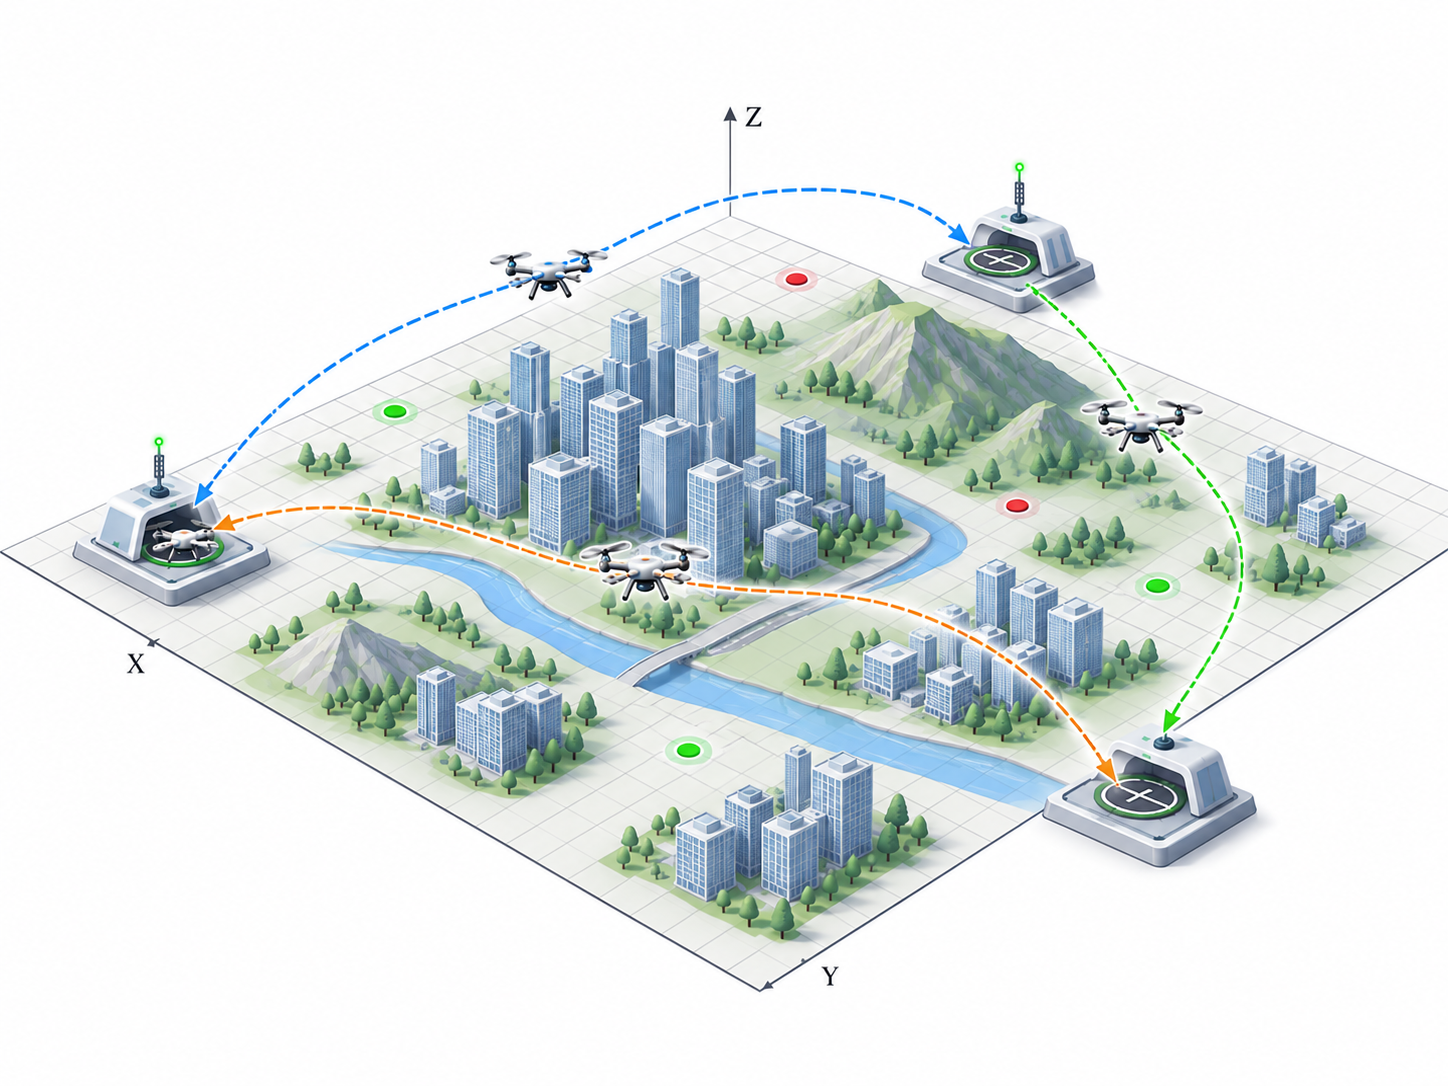
\includegraphics[width=0.6\textwidth]{figures/fig1-Illustration-of-a-motivating-scenario-for-multi-UAV-and-multi-depot.png}
      \caption{多机巢下无人机协同作业场景}\label{fig:frame}
\end{figure}
任务沿时间轴持续到达，机队持续运转，机巢分散部署；无人机自机巢起飞执行任务，完成后降落于某一可用机巢。由于任务到达速率与机队服务能力不匹配，任务池通常无法被全部覆盖。本文将其刻画为滚动时域下的选择性多机巢多无人机任务分配问题，按固定周期序贯决策。文中主要符号见表~\ref{tab:symbols}，周期下标 $t$ 在不引起混淆时省略。建模假设如下：
\begin{enumerate}[label=(\arabic*), leftmargin=3.5em]
      \item 任务的到达时刻、位置、收益及服务期限由外生过程给定，本文不对其作预测；决策按周期推进，每周期初规划、周期内执行、周期末反馈。周期内实时航迹与冲突不予建模，单周期子问题为静态组合优化；问题的动态性体现于任务池演化与跨周期状态继承。
      \item 任务池整体超出当期机队服务能力，供不应求为常态；据此不要求任务全集可被交付，未接纳者留池，于后续周期继续参与分配。
      \item 机队允许异构，各机满电航程 $B_u^{\max}$、巡航速度 $v_u$ 与最大飞行时间 $T_u^{\max}$ 可互不相同，其余能力参数一致；各机每周期至多出动一个航次，返航后降落于机巢并换电，剩余航程恢复至该机满电航程。跨周期耦合体现于终点机巢位置、机队可用性与任务池演化，航程约束以各机当期剩余航程 $B_u(t)$ 为基准，更新见式~\eqref{eq:range_update}。
      \item 各节点之间的飞行代价取三维航程估计。估计时沿两节点水平投影作垂直切面，取地形与建筑屋顶构成的障碍包络，按最小离地间隙与爬升斜率生成地形跟随估计航迹，以其长度作为该段航程。该估计为全文统一的代价口径，未计入飞行动力学与可飞性约束，不等同于欧氏距离且一般非对称；目标与航程约束共用该代价矩阵。
\end{enumerate}

单周期 $t$ 的输入为任务池 $\mathcal{T}_t=\mathcal{T}_t^{\mathrm{remain}}\cup\mathcal{T}_t^{\mathrm{new}}\cup\mathcal{T}_t^{\mathrm{release}}$，三子集依次为滞留、新到达与故障释放任务；机队状态 $\mathcal{U}_t$ 含位置、剩余航程与可用性；机巢集合 $\mathcal{N}$ 含位置、容量占用与可用性。输出为接纳集 $\mathcal{T}_t^{\mathrm{sel}}$、执行集 $\mathcal{T}_t^{\mathrm{exec}}$、各机访问顺序 $\pi_u$ 与各航次终点机巢 $\nu_u$，由决策变量 $z_j$、$y_j$、$x_{uj}$、$\pi_u$、$\nu_u$ 确定，且 $\mathcal{T}_t^{\mathrm{exec}}\subseteq\mathcal{T}_t^{\mathrm{sel}}\subseteq\mathcal{T}_t$。未执行任务与演化后的机队状态传递至下一周期。

\begin{table}[htbp]
      \centering
      \caption{主要符号及其含义}\label{tab:symbols}
      \begin{tabularx}{\textwidth}{lXlX}
            \toprule
            符号                                                             & 含义                                   & 符号                                                                                                  & 含义                              \\
            \midrule
            \multicolumn{4}{l}{\emph{集合与索引}}                                                                                                                                                                                                              \\
            $\mathcal{T}_t$                                                & 周期 $t$ 的任务池                          & $\mathcal{T}_t^{\mathrm{remain}},\ \mathcal{T}_t^{\mathrm{new}},\ \mathcal{T}_t^{\mathrm{release}}$ & 任务池的滞留、新到达与故障释放子集               \\
            $\mathcal{T}_t^{\mathrm{loadable}}$                            & 任务池中硬约束下存在可行航次的任务集                   & $\mathcal{U}_t,\ \mathcal{U}_t^{\mathrm{avail}},\ \mathcal{N}$                                      & 无人机集合、可用子集与机巢集合                 \\
            $j,\ u,\ n$                                                    & 任务、无人机、机巢的索引                         & $\prec$                                                                                             & 任务之间的时序先后关系                     \\
            \midrule
            \multicolumn{4}{l}{\emph{外生参数}}                                                                                                                                                                                                               \\
            $\bm{p}_j$                                                     & 任务 $j$ 的位置向量                         & $R_j$                                                                                               & 任务 $j$ 的收益，仅用于事后评价              \\
            $a_j$                                                          & 任务 $j$ 的到达时刻                         & $e_j,\ l_j$                                                                                         & 期望服务期限的下界与上界；迟到允许并计价            \\
            $\bm{p}_u(t),\ B_u(t)$                                         & 周期 $t$ 无人机 $u$ 的位置与剩余航程              & $v_u,\ B_u^{\max},\ T_u^{\max},\ s_j$                                                               & 各机巡航速度、满电航程与最大飞行时间；任务 $j$ 的服务时长 \\
            $\bm{p}_n,\ C_n,\ \delta_n(t)$                                 & 机巢 $n$ 的位置、停机位容量与可用性                 & $c(\bm{p},\bm{p}\,')$                                                                               & 节点间三维航程估计，一般非对称                 \\
            $w_{\mathrm{late}}$                                            & 迟到量的单位计价系数                           & $\lambda$                                                                                           & 三维航程的成本系数                       \\
            $\sigma_t$                                                     & 本周期接纳名额上界，估计口径见第~3~节                 &                                                                                                     &                                 \\
            \midrule
            \multicolumn{4}{l}{\emph{决策变量}}                                                                                                                                                                                                               \\
            $z_j$                                                          & 任务 $j$ 是否被接纳                         & $x_{uj}$                                                                                            & 任务 $j$ 是否指派给无人机 $u$             \\
            $y_j$                                                          & 任务 $j$ 是否于本周期执行                      & $\pi_u$                                                                                             & 无人机 $u$ 航次内任务的访问顺序              \\
            $\nu_u$                                                        & 无人机 $u$ 航次的终点机巢                      &                                                                                                     &                                 \\
            \midrule
            \multicolumn{4}{l}{\emph{导出量}}                                                                                                                                                                                                                \\
            $\mathcal{T}_t^{\mathrm{sel}},\ \mathcal{T}_t^{\mathrm{exec}}$ & 接纳集 $\{j:z_j=1\}$ 与执行集 $\{j:y_j=1\}$ & $T_j$                                                                                               & 任务 $j$ 的完成时刻                    \\
            $L_j=\max(0,\ T_j-l_j)$                                        & 任务 $j$ 的迟到量                          & $L_{\mathrm{tot}}=\sum_{j\in\mathcal{T}_t^{\mathrm{exec}}}L_j$                                      & 单周期总迟到量                         \\
            $d_u(\pi_u,\nu_u)$                                             & 无人机 $u$ 航次含返航的三维总航程                  & $\tau_u(\pi_u,\nu_u)$                                                                               & 无人机 $u$ 航次含返航的飞行时长              \\
            $C_n^{\mathrm{free}}(t)$                                       & 机巢 $n$ 的可用停机位，$C_n-o_n+q_n$          &                                                                                                     &                                 \\
            \bottomrule
      \end{tabularx}
\end{table}

\subsection{约束条件}

单周期约束含单机、结构、时序与机巢四类硬约束，另设软时间窗，时间窗违约计入目标而不进入硬不可行集。以下仅对可用机 $u\in\mathcal{U}^{\mathrm{avail}}$ 构造航次。

\subsubsection*{单机约束}

无人机 $u$ 自 $\bm{p}_u$ 出发，按 $\pi_u$ 依次服务任务后降落于 $\nu_u$。含返航的总航程 $d_u(\pi_u,\nu_u)$ 沿非对称代价 $c(\cdot,\cdot)$ 累加，飞行时长 $\tau_u=d_u/v_u$。硬资源约束为
\begin{equation}
      d_u(\pi_u,\nu_u) \le B_u(t),
      \qquad
      \tau_u(\pi_u,\nu_u) \le T_u^{\max},
      \qquad \forall u\in\mathcal{U}^{\mathrm{avail}},
      \label{eq:range_time}
\end{equation}
其中 $B_u(t)$ 为该机当期剩余航程，未必等于满电航程；$T_u^{\max}$ 可由 $B_u^{\max}$ 与 $v_u$ 派生，亦可取更紧的经验上界。越界航次物理不可行，空航次不计航程与时长。因每航次均降落于机巢并换电，状态更新为
\begin{equation}
      B_u(t+1)=
      \begin{cases}
            B_u^{\max}, & \text{本周期出动},  \\
            B_u(t),     & \text{本周期不出动},
      \end{cases}
      \qquad
      \bm{p}_u(t+1)=\bm{p}_{\nu_u}.
      \label{eq:range_update}
\end{equation}

\subsubsection*{结构约束}

接纳、执行与指派的逻辑关系为
\begin{equation}
      y_j \le z_j, \qquad
      \sum_{u\in\mathcal{U}^{\mathrm{avail}}} x_{uj} = y_j,
      \qquad
      z_j,\, y_j,\, x_{uj}\in\{0,1\},
      \qquad \forall j\in\mathcal{T}_t,\ \forall u\in\mathcal{U}^{\mathrm{avail}};
      \quad
      \sum_{j\in\mathcal{T}_t} z_j \le \sigma_t.
      \label{eq:assign_link}
\end{equation}
即未接纳不得执行，执行当且仅当由一架可用机承担；接纳总数不超过本周期名额上界 $\sigma_t$，且接纳仅在 $\mathcal{T}_t^{\mathrm{loadable}}$ 内进行。$\pi_u$ 为 $\{j:x_{uj}=1\}$ 上的排列，允许空排列。

\subsubsection*{时序约束}

部分任务带先后关系 $j\prec j'$，该关系仅在航次内生效。当 $j$ 与 $j'$ 由同一架机在同一航次承载时，$j$ 须先于 $j'$ 完成，
\begin{equation}
      x_{uj}=x_{uj'}=1\ \Longrightarrow\ T_j\le T_{j'},\qquad
      \forall u\in\mathcal{U}^{\mathrm{avail}},\ j\prec j'.
      \label{eq:prec_order}
\end{equation}
跨机、跨周期的绝对时序与多机协同到达超出本文范围，不作约束。

同一时序链内的任务另受原子性约束，整链作为不可拆分的调度单元，本周期要么整组执行并同周期交付，要么整组留池。链中部分任务被执行不构成时序违约，却会在准入与交付环节被整组剔除；组内任务可不同机。

\subsubsection*{机巢约束}

$\nu_u$ 为决策变量，可取任一可用机巢。记 $o_n(t)$ 为周期初归属 $n$ 的机数，$q_n(t)$ 为自 $n$ 起飞的机数，终点可用停机位为
\begin{equation}
      C_n^{\mathrm{free}}(t)=C_n-o_n(t)+q_n(t),
      \label{eq:free_slot}
\end{equation}
终点选择须满足
\begin{equation}
      \sum_{u\in\mathcal{U}^{\mathrm{avail}}} \mathbf{1}\{\nu_u = n\}
      \le C_n^{\mathrm{free}}(t),
      \qquad
      \nu_u \in \{n\in\mathcal{N}:\delta_n(t)=1\}.
      \label{eq:nest_cap}
\end{equation}
停机位按周期末归属在决策时预占，起飞释放与终点占位同时计入，他巢起飞而降落本巢亦不致超容；末任务至 $\nu_u$ 的返航段须在代价矩阵上可达，且已计入 $d_u$ 与 $\tau_u$。容量在全队终点选择上耦合，故终点决策须在航次给定后联合求解，见第~3~节。

\subsubsection*{软时间窗约束}

任务 $j$ 的服务窗为 $[e_j,l_j]$，迟到允许且不设硬上限，按 $w_{\mathrm{late}}$ 折价计入目标。设 $\pi_u=(j_1,\dots,j_m)$，本周期出发时刻为 $t_0$，任务 $j$ 的服务时长为 $s_j$。完成时刻沿航次递推：
\begin{equation}
      T_{j_k}=\max\!\bigl(T_{j_{k-1}}+c(\bm{p}_{j_{k-1}},\bm{p}_{j_k})/v_u,\ e_{j_k}\bigr)+s_{j_k},
      \qquad T_{j_0}=t_0,\ \bm{p}_{j_0}=\bm{p}_u,
      \label{eq:completion}
\end{equation}
故早到等待与服务时长均计入完成时刻。迟到量 $L_j=\max(0,T_j-l_j)$，总迟到量 $L_{\mathrm{tot}}$ 进入式~\eqref{eq:obj}；服务窗只影响计价，不改变可行域。

\subsection{优化模型与问题性质}

记 $\mathcal{T}_t^{\mathrm{loadable}}\subseteq\mathcal{T}_t$ 为任务池中在式~\eqref{eq:range_time}--\eqref{eq:nest_cap} 下存在可行航次、可被本周期机队服务的任务集，其余任务不作本周期承诺，留池顺延。由假设 (2)，可服务任务通常多于本周期名额，不能要求其全部交付；故目标分两层：先在名额与硬约束下最大化本周期交付数，再在不降低该交付数的前提下最小化迟到与航程。采用两阶段形式书写，第一层为
\begin{equation*}
      \begin{aligned}
            (P_1)\quad \max\quad & \sum_{j\in\mathcal{T}_t} y_j                                                                                                \\
            \text{s.t.}\quad     & \sum_{j\in\mathcal{T}_t} z_j \le \sigma_t,\quad y_j\le z_j,\ \forall j\in\mathcal{T}_t,                                     \\
                                 & \text{式~\eqref{eq:range_time}--\eqref{eq:nest_cap}、\eqref{eq:assign_link} 成立，且 $\pi_u$ 为执行集上的排列并满足式~\eqref{eq:prec_order}。}
      \end{aligned}
\end{equation*}
其中名额 $\sigma_t$ 由当期机队剩余航程与单任务代价估计给出，仅作接纳数上界而非等式：估计偏高时，第一层的最优值自动退化为机队真实可达的交付上限，模型不会因此不可行。记 $(P_1)$ 的最优值为 $Y_t^*$；将其作为 $\varepsilon$-约束代入第二层，得到唯一的目标函数式
\begin{equation}
      \begin{aligned}
            (P_2)\quad \min\quad
             & w_{\mathrm{late}} L_{\mathrm{tot}}
            +\lambda\sum_{u\in\mathcal{U}^{\mathrm{avail}}}d_u(\pi_u,\nu_u)                                                                \\
            \text{s.t.}\quad
             & \sum_{j\in\mathcal{T}_t} y_j \ge Y_t^*,                                                                                     \\
             & \text{式~\eqref{eq:range_time}--\eqref{eq:nest_cap}、\eqref{eq:assign_link} 成立，且 $\pi_u$ 为执行集上的排列并满足式~\eqref{eq:prec_order}。}
      \end{aligned}
      \label{eq:obj}
\end{equation}
$P_1$ 的最优值以 $\varepsilon$-约束进入 $P_2$，故两阶段与「先比覆盖、再比成本」的字典序等价，且全文仍只有式~\eqref{eq:obj} 一个目标函数式，不必引入字典序记号。第一层压满的是交付数 $\sum_j y_j$ 而非接纳数 $\sum_j z_j$：名额用满只保证接纳集规模，唯有交付数取到 $Y_t^*$ 才使覆盖落地；受硬约束限制而无法于本周期交付的可服务任务不作承诺、留池顺延，不视为违约。收益 $R_j$ 不参与解的取舍，不入目标，仅用于事后评价；$z$ 为独立的取舍维度，由名额上界与第一层共同确定，不再是可行域的派生量。目标两项量纲不同，$\lambda$ 为每米航程的成本系数，$w_{\mathrm{late}}$ 为每单位迟到时间的里程当量，二者按此口径标定后相加，取值见第~4~节。

需强调，$(P_1)$ 与 $(P_2)$ 是同一单周期问题两层目标的分层表述：二者经 $\varepsilon$-约束相联系，并非按时间先后执行的两个求解步骤，也不对应第~3~节「阶段一接纳、阶段二分配」的求解框架划分。本文所称「字典序」仅指上述目标优先序，用于界定最优解的含义；实际求解时由覆盖门禁与支配权重把覆盖优先嵌入单一适应度标量，并不显式求解 $Y_t^*$。故第~3~节描述的是该优先序的实现方式，而非 $(P_1)$、$(P_2)$ 的依次求解。

该问题的组合规模为指数级。任务取舍对应 $2^{|\mathcal{T}_t|}$ 个子集，指派与访问顺序构成阶乘级排列，终点机巢又在全队容量上耦合。若限定单一机巢并固定返回、令名额上界不小于任务全集使第一层退化为覆盖全集、航程退化为平面代价，且令 $w_{\mathrm{late}}\to\infty$ 使软时间窗退化为硬时间窗，则 $(P_2)$ 在交付全集下退化为带时间窗的车辆路径问题；该特例已知为 NP 难，故本文单周期问题亦为 NP 难。上述决策相互耦合，精确联合求解难以在周期时限内完成，第~3~节据此采用选择—分配—滚动的分层框架，以放弃全局最优性保证换取可扩展性。

本文取单周期视界，跨周期仅通过机队状态与任务池演化耦合，不作多周期前瞻。任务完成按周期末统一结算，$T_j$ 用于迟到计价与航序判据，不驱动状态转移。

